\chapter{Sistemas con restricciones y movimiento hamiltoniano}

\lectureoverview{Dos sistemas con restricciones muestran por qué la mecánica lagrangiana es tan eficaz: una vez elegidas coordenadas adecuadas, las ecuaciones de movimiento y sus leyes de conservación se obtienen sin calcular explícitamente las fuerzas de restricción. Estos mismos ejemplos conducen después a la mecánica hamiltoniana, en la que las coordenadas y los momentos forman el espacio de fases, el oscilador armónico se convierte en una rotación rígida y las dos ecuaciones de primer orden de Hamilton sustituyen a cada ecuación de Euler--Lagrange de segundo orden.}

\section{Qué significa resolver un problema de mecánica}

El propósito inmediato del método lagrangiano es práctico. Tanto una cuña que se desliza sobre un suelo como un péndulo doble pueden tratarse con las leyes de Newton, pero las fuerzas de contacto y las tensiones desconocidas pronto vuelven engorrosos los cálculos. Una vez conocidas las reglas de la mecánica lagrangiana, los mismos problemas se resuelven mediante una sucesión de pasos controlados:
\begin{enumerate}
  \item elegir coordenadas independientes que describan una configuración instantánea;
  \item expresar las energías cinética y potencial en esas coordenadas;
  \item formar \(L=T-V\) y aplicar las ecuaciones de Euler--Lagrange.
\end{enumerate}

Para lo que nos ocupa, un problema ya está \emph{resuelto} cuando se han escrito correctamente sus ecuaciones de movimiento. Aún se puede buscar una trayectoria en forma cerrada, pero esa es otra cuestión. Una vez completado el planteamiento mecánico, las ecuaciones diferenciales no lineales pueden integrarse numéricamente. La parte difícil a menudo no es la integración, sino encontrar variables que incorporen las restricciones sin introducir fuerzas desconocidas redundantes.

\section{Una partícula que se desliza sobre una cuña móvil}

Consideremos una cuña de masa \(M\), con la restricción de deslizarse sin fricción sobre un plano horizontal. Una partícula puntual de masa \(m\) está restringida a permanecer sobre la cara inclinada. Hay dos grados de libertad: uno indica la posición de la cuña y el otro, la posición de la partícula sobre ella.

Sea
\begin{equation}
  \begin{aligned}
    X&=\text{horizontal position of the wedge corner},\\
    x&=\text{horizontal displacement of the particle}\\[-0.2em]
     &\phantom{={}}\text{from that corner}.
  \end{aligned}
  \label{eq:l6-wedge-coordinates}
\end{equation}
Por tanto, la coordenada horizontal absoluta de la partícula es \(X+x\). La elección no es única. También podríamos usar la distancia a lo largo de la pendiente o la coordenada horizontal absoluta de la partícula. Cualquier par no redundante que describa las mismas configuraciones es válido, aunque algunos pares hacen más patente la estructura que otros.

Para un ángulo fijo de la pendiente \(\beta\), el desplazamiento vertical \(y\) no es una coordenada independiente:
\begin{equation}
  y=x\tan\beta,
  \qquad
  \dot y=\dot x\tan\beta.
  \label{eq:l6-wedge-constraint}
\end{equation}
Nos restringimos al caso \(\beta=45^\circ\), de modo que \(y=x\) y
\(\dot y=\dot x\). Esta simplificación elimina los factores trigonométricos sin alterar el propósito del ejemplo.

\begin{figure}[htbp]
  \centering
  \includegraphics[width=0.84\textwidth]{lecture_06_figure_06.png}
  \caption{La cuña móvil, la partícula restringida y las componentes horizontal y vertical de la velocidad que se utilizan en el ejemplo de \(45^\circ\).}
  \lectureframe{00:10:25}
\end{figure}

La energía cinética de la cuña es
\begin{equation}
  T_{M}=\frac{M}{2}\dot X^2.
  \label{eq:l6-wedge-kinetic}
\end{equation}
La velocidad horizontal de la partícula es \(\dot X+\dot x\), mientras que su velocidad vertical es \(\dot x\). Por consiguiente, su energía cinética es
\begin{equation}
  T_m=\frac{m}{2}\left[(\dot X+\dot x)^2+\dot x^2\right].
  \label{eq:l6-particle-kinetic}
\end{equation}
Si fijamos el cero de la energía potencial gravitatoria en \(x=0\), tenemos \(V=mgx\). Así,
\begin{equation}
  L=\frac{M}{2}\dot X^2
    +\frac{m}{2}\left[(\dot X+\dot x)^2+\dot x^2\right]
    -mgx.
  \label{eq:l6-wedge-lagrangian}
\end{equation}

\begin{figure}[htbp]
  \centering
  \includegraphics[width=0.86\textwidth]{lecture_06_figure_07.png}
  \caption{La geometría de la cuña, \(V=mgx\), y las dos contribuciones a la energía cinética reunidas en la pizarra.}
  \lectureframe{00:14:15}
\end{figure}

\subsection{El momento canónico se define a partir del lagrangiano}

Los momentos canónicos se definen a partir del lagrangiano, no mediante una conjetura basada en la velocidad de una sola partícula:
\begin{align}
  p_X&=\frac{\partial L}{\partial\dot X}
      =M\dot X+m(\dot X+\dot x),
      \label{eq:l6-wedge-pX}\\
  p_x&=\frac{\partial L}{\partial\dot x}
      =m(\dot X+\dot x)+m\dot x.
      \label{eq:l6-wedge-px}
\end{align}
La primera expresión es el momento horizontal total ordinario: la cuña aporta \(M\dot X\) y la partícula aporta \(m(\dot X+\dot x)\). Aquí aparece como el momento conjugado de la coordenada \(X\).

\begin{figure}[htbp]
  \centering
  \includegraphics[width=0.86\textwidth]{lecture_06_figure_08.png}
  \caption{Los momentos canónicos conjugados a la coordenada de la cuña \(X\) y a la coordenada relativa de la partícula \(x\).}
  \lectureframe{00:18:05}
\end{figure}

El lagrangiano no depende explícitamente de \(X\). Una traslación horizontal de todo el dispositivo transforma las coordenadas así:
\begin{equation}
  \delta X=\epsilon,
  \qquad
  \delta x=0.
  \label{eq:l6-wedge-translation}
\end{equation}
Por tanto, la regla general para una simetría infinitesimal
\begin{equation}
  \delta q_i=\epsilon f_i(q),
  \qquad
  Q=\sum_i p_i f_i
  \label{eq:l6-noether-rule}
\end{equation}
da \(Q=p_X\). Equivalentemente, \(X\) es cíclica y
\begin{equation}
  \dot p_X=\frac{\partial L}{\partial X}=0.
  \label{eq:l6-wedge-conservation}
\end{equation}

No hay una simetría correspondiente de traslación vertical. La cuña no puede moverse verticalmente, y un cambio en la altura de la partícula modifica la energía potencial gravitatoria. El momento horizontal se conserva; el momento vertical de este subsistema con restricciones no se conserva.

Para la coordenada relativa, la ecuación de Euler--Lagrange es
\begin{equation}
  \dot p_x=\frac{\partial L}{\partial x}=-mg.
  \label{eq:l6-wedge-force}
\end{equation}
Hubo que corregir un signo en esta línea en la pizarra. El procedimiento fiable consiste en partir de \(L=T-V\): como \(V=mgx\), la derivada del lagrangiano es \(-mg\). Que \(x\) se haya introducido como desplazamiento horizontal no elimina la gravedad de su ecuación, porque la restricción relaciona ese desplazamiento horizontal con la altura vertical \(y=x\).

No ha aparecido ninguna fuerza normal ni de reacción. Esas fuerzas toman los valores necesarios para mantener las restricciones. El método de Newton las introduciría y las calcularía junto con las aceleraciones; las coordenadas generalizadas han hecho innecesario hacerlo.

\section{El péndulo doble y el arte de elegir coordenadas}

Suspendamos ahora dos masas unitarias de dos varillas sin masa y de longitud unidad. La primera varilla forma un ángulo \(\theta\) con la vertical hacia abajo. Para el segundo grado de libertad, podemos elegir entre dos opciones. Podríamos usar un segundo ángulo absoluto \(\phi\) o el ángulo relativo \(\alpha\) entre las varillas.

El ángulo relativo es la opción más reveladora. Desactivemos momentáneamente la gravedad. Una rotación rígida del aparato completo cambia su orientación absoluta, pero no el ángulo entre las varillas:
\begin{equation}
  \theta\longrightarrow\theta+\epsilon,
  \qquad
  \alpha\longrightarrow\alpha.
  \label{eq:l6-double-rotation}
\end{equation}
Con esta elección, la simetría rotacional actúa sobre una sola coordenada. Esto no significa que otros sistemas de coordenadas sean incorrectos. Significa que la simetría y, por tanto, la cantidad conservada se ven con mayor facilidad.

\begin{figure}[htbp]
  \centering
  \includegraphics[width=0.76\textwidth]{lecture_06_figure_09.png}
  \caption{El péndulo doble, con \(\theta\) como primer ángulo absoluto y \(\alpha\) como ángulo de la segunda varilla respecto de la primera.}
  \lectureframe{00:29:20}
\end{figure}

Para obtener la energía cinética, usemos coordenadas cartesianas como recurso auxiliar de cálculo. Si medimos la coordenada vertical hacia abajo, la primera masa pendular está en
\begin{equation}
  x_1=\sin\theta,
  \qquad
  y_1=\cos\theta,
  \label{eq:l6-bob-one-position}
\end{equation}
y, por tanto,
\begin{equation}
  \dot x_1=\dot\theta\cos\theta,
  \qquad
  \dot y_1=-\dot\theta\sin\theta,
  \qquad
  \dot x_1^2+\dot y_1^2=\dot\theta^2.
  \label{eq:l6-bob-one-velocity}
\end{equation}
La segunda masa pendular está en
\begin{align}
  x_2&=\sin\theta+\sin(\theta+\alpha),\\
  y_2&=\cos\theta+\cos(\theta+\alpha),
  \label{eq:l6-bob-two-position}
\end{align}
y, por ejemplo,
\begin{equation}
  \dot x_2=\dot\theta\cos\theta
  +(\dot\theta+\dot\alpha)\cos(\theta+\alpha),
  \label{eq:l6-bob-two-xvelocity}
\end{equation}
con una expresión análoga para \(\dot y_2\).

\begin{figure}[htbp]
  \centering
  \includegraphics[width=0.88\textwidth]{lecture_06_figure_10.png}
  \caption{Coordenadas cartesianas auxiliares para las dos masas pendulares. Se usan para calcular las velocidades, no se introducen como grados de libertad adicionales.}
  \lectureframe{00:35:25}
\end{figure}

Al sumar las dos energías cinéticas se obtiene el resultado coherente que sigue. El término cruzado se deduce de
\begin{equation*}
  \cos A\cos B+\sin A\sin B=\cos(A-B).
\end{equation*}
\begin{equation}
  T=\dot\theta^2
    +\frac12(\dot\theta+\dot\alpha)^2
    +\dot\theta(\dot\theta+\dot\alpha)\cos\alpha.
  \label{eq:l6-double-kinetic}
\end{equation}

\begin{classroomqa}
  \audiencequestion{¿Esta expresión ya incluye la energía cinética de las dos masas pendulares, o se ha perdido un factor de un medio?
  \lecturetimestamp{00:38:06--00:38:27}}
  \lecturerresponse{Incluye la de ambas. Se obtiene de
  \(\tfrac12(\dot x_1^2+\dot y_1^2+\dot x_2^2+\dot y_2^2)\).
  Las dos contribuciones iguales se combinan para dar el primer término
  \(\dot\theta^2\); no falta ningún factor.}
\end{classroomqa}

Sin gravedad, \(L=T\) no depende explícitamente de \(\theta\). Por tanto,
\begin{equation}
  \dot p_\theta=\frac{\partial L}{\partial\theta}=0,
  \label{eq:l6-double-angular-conservation}
\end{equation}
y \(p_\theta\) es el momento angular total. Obsérvese el significado preciso de la afirmación de que \(\theta\) no aparece: \(\dot\theta\) sí aparece, pero la coordenada sin derivar no.

Al restablecer la gravedad, se rompe la simetría rotacional global. Con la convención de la vertical hacia abajo usada antes, una elección conveniente del cero da
\begin{equation}
  V=-g(y_1+y_2)
   =-g\left[2\cos\theta+\cos(\theta+\alpha)\right].
  \label{eq:l6-double-potential}
\end{equation}
Una constante aditiva no cambiaría nada. Lo importante es que ahora \(\theta\) aparece explícitamente, por lo que su momento conjugado deja de conservarse. La energía se conserva porque el lagrangiano no depende explícitamente del tiempo.

\begin{classroomqa}
  \audiencequestion{¿Debería ser \(\dot\theta-\dot\alpha\) en la pizarra
  \(\dot\theta+\dot\alpha\)?
  \lecturetimestamp{00:43:00--00:43:54}}
  \lecturerresponse{La orientación usada aquí requiere el signo más. Es la convención de la ecuación~\eqref{eq:l6-bob-two-position}, que se mantiene en la energía cinética de la ecuación~\eqref{eq:l6-double-kinetic}. Invertir la definición del sentido positivo de \(\alpha\) cambia los signos correspondientes, pero entonces hay que cambiar de manera coherente todas sus apariciones. En la pizarra se mezclaron las dos convenciones.}
\end{classroomqa}

\begin{figure}[htbp]
  \centering
  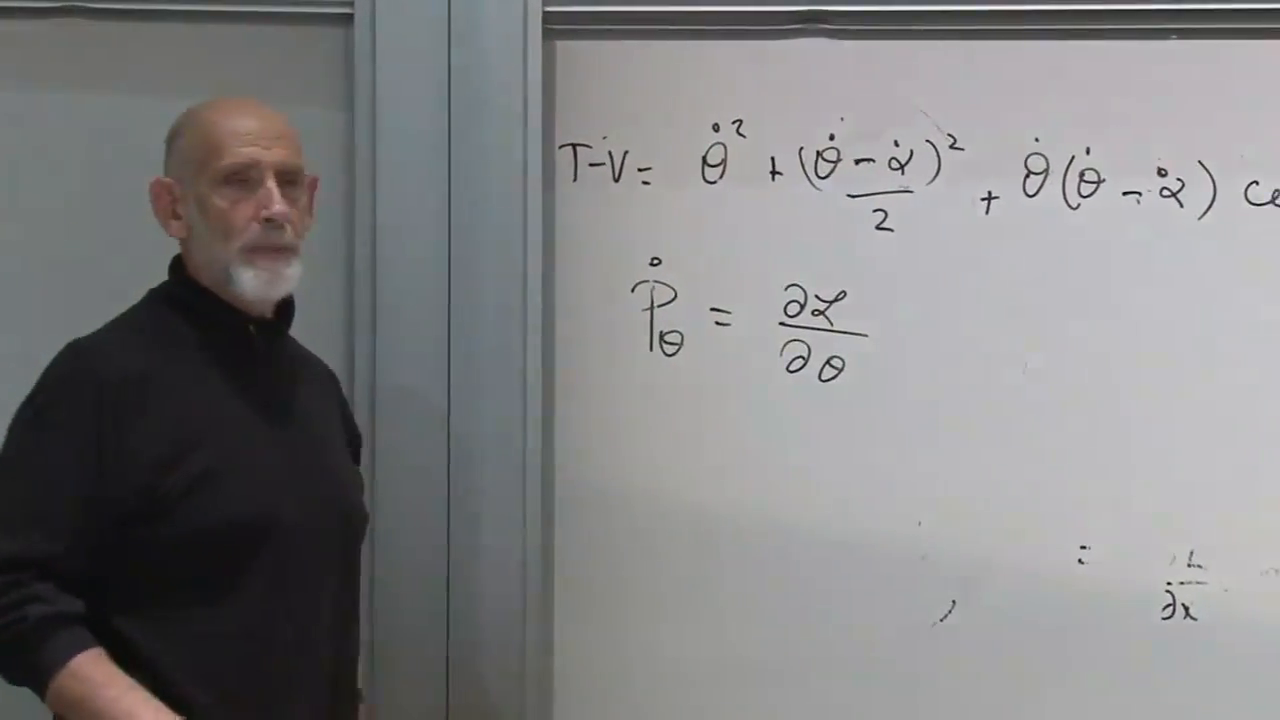
\includegraphics[width=0.84\textwidth]{lecture_06_figure_02.png}
  \caption{El cálculo del péndulo sin gravedad y \(\dot p_\theta=\partial L/\partial\theta\). La línea superior de la pizarra conserva la notación local con signos incoherentes que se comenta en la pregunta; la fórmula normalizada es la ecuación~\eqref{eq:l6-double-kinetic}.}
  \lectureframe{00:45:50}
\end{figure}

Una vez conocidos \(T\) y \(V\), las ecuaciones restantes se obtienen por derivación. Las tensiones de las varillas y las fuerzas que imponen longitudes fijas también han desaparecido gracias a la elección de coordenadas.

\subsection{Qué implica y qué no implica la conservación}

\begin{classroomqa}
  \audiencequestion{¿Se puede saber directamente por las ecuaciones si el péndulo doble es caótico?
  \lecturetimestamp{00:44:57--00:45:25}}
  \lecturerresponse{Por lo general, no mediante una inspección sencilla. Al variar los parámetros o las energías, un sistema puede pasar de un comportamiento regular a uno caótico. Este tema requiere más estructura que la que revela el aspecto inmediato de las ecuaciones y se abordará más adelante.}
\end{classroomqa}

\begin{classroomqa}
  \audiencequestion{En un sistema conservativo, ¿todo \(\dot p_i\) es igual a cero?
  \lecturetimestamp{00:45:25--00:46:24}}
  \lecturerresponse{No. La ecuación general es \(\dot p_i=\partial L/\partial q_i\). Solo se anula cuando \(q_i\) es cíclica. Una coordenada cíclica es el caso especialmente sencillo en que una simetría se expresa como un desplazamiento de una coordenada que deja fijas las demás.}
\end{classroomqa}

Si el único objetivo es obtener la evolución numérica, también sirve un sistema de coordenadas poco conveniente; simplemente produce ecuaciones más largas. La ventaja de elegir un sistema ingenioso es conceptual: el momento conservado queda a la vista antes de resolver las ecuaciones.

\begin{classroomqa}
  \audiencequestion{Sin gravedad, ¿se comporta un péndulo doble con la misma sencillez que un péndulo libre simple?
  \lecturetimestamp{00:47:02--00:47:35}}
  \lecturerresponse{Un rotor libre simple gira uniformemente porque su único momento angular determina su movimiento. Un péndulo doble puede ejecutar movimientos relativos muy complicados mientras conserva el momento angular total. Si ambas velocidades angulares son inicialmente nulas, permanece en reposo; de lo contrario, las dos partes interactúan.}
\end{classroomqa}

\begin{classroomqa}
  \audiencequestion{En ausencia de gravedad, ¿son constantes por separado \(\dot\theta\) y \(\dot\alpha\)?
  \lecturetimestamp{00:47:36--00:52:42}}
  \lecturerresponse{No. La conservación indica \(\dot p_\theta=0\), no \(\ddot\theta=0\) ni \(\ddot\alpha=0\). La expresión de \(p_\theta=\partial L/\partial\dot\theta\) contiene ambas velocidades angulares y depende de \(\alpha\). Las varillas transmiten torques, lo que permite que las dos masas pendulares intercambien momento angular y energía. Esto es análogo a dos masas unidas por un resorte: el momento total y la velocidad del centro de masa son constantes, mientras que las velocidades individuales oscilan. El análogo rotacional es una combinación colectiva particular, no ninguno de los dos ángulos por separado.}
\end{classroomqa}

\begin{classroomqa}
  \audiencequestion{¿Las fuerzas que intercambian momento angular se transmiten a través de las varillas?
  \lecturetimestamp{00:52:43--00:53:34}}
  \lecturerresponse{Sí. Una fuerza transmitida a lo largo de una varilla no tiene por qué pasar por el pivote del otro movimiento, así que puede ejercer un torque. Un torque es simplemente la tendencia de una fuerza a producir rotación y, en este caso, genera aceleraciones angulares individuales no nulas.}
\end{classroomqa}

\section{El hamiltoniano como tercera formulación}

El hamiltoniano es la energía, pero esa es solo su primera acepción. También constituye la base de una tercera formulación de la mecánica. Las ecuaciones de Newton usan fuerzas y aceleraciones. El principio de acción estacionaria da las ecuaciones de Euler--Lagrange. La mecánica hamiltoniana es equivalente a esta última para sistemas regulares, pero sus variables y su geometría son diferentes.

En lugar de \(q_i\) y \(\dot q_i\), usemos \(q_i\) y sus momentos conjugados \(p_i\). Para describir el estado de un sistema con \(n\) grados de libertad se necesitan \(2n\) números en cualquiera de las dos formulaciones: posiciones y velocidades, o posiciones y momentos. La relación entre ambas es
\begin{equation}
  p_i=\frac{\partial L}{\partial\dot q_i}.
  \label{eq:l6-legendre-map}
\end{equation}
Cuando estas relaciones se pueden invertir para despejar las velocidades \(\dot q_i(q,p)\), definimos
\begin{equation}
  H(q,p)=\sum_i p_i\dot q_i-L(q,\dot q).
  \label{eq:l6-hamiltonian-definition}
\end{equation}
A continuación se eliminan las velocidades del lado derecho en favor de \(q\) y \(p\). Esta invertibilidad es la hipótesis de regularidad de la transformación de Legendre. Los lagrangianos singulares requieren la teoría más general de sistemas con restricciones; esta construcción elemental no los trata.

\subsection{La reversibilidad antes del cálculo}

Recordemos una colección finita de estados abstractos conectados por flechas. Aunque una regla sea determinista, puede no ser reversible si dos estados anteriores conducen a uno posterior. El futuro es único, pero el pasado no. Al invertir todas las flechas se obtiene el defecto opuesto: un estado se ramifica en varios futuros. En el primer diagrama las flechas convergen; en el segundo divergen.

\begin{figure}[htbp]
  \centering
  \includegraphics[width=0.86\textwidth]{lecture_06_figure_11.png}
  \caption{Mapas abstractos de estados que contrastan los ciclos reversibles con la convergencia y la divergencia prohibidas.}
  \lectureframe{00:56:20}
\end{figure}

El flujo hamiltoniano proporcionará la versión continua de esta afirmación. Una nube de puntos del espacio de fases puede desplazarse y deformarse, pero no puede adquirir un sumidero que destruya las diferencias entre estados, ni una fuente que genere varios futuros a partir de un solo estado. Dejaremos la demostración para más adelante; por ahora, los diagramas sirven para motivar la geometría.

\begin{classroomqa}
  \audiencequestion{¿Debe interpretarse el diagrama abstracto de estados como un objeto que se mueve en un campo gravitatorio?
  \lecturetimestamp{00:58:02--00:58:35}}
  \lecturerresponse{No. Los puntos representan simplemente estados abstractos y las flechas especifican una regla para cambiar de estado. Al dibujo no se le ha asignado ningún significado espacial ni gravitatorio.}
\end{classroomqa}

\begin{classroomqa}
  \audiencequestion{¿En qué se distingue un mapa convergente de estados, que está prohibido, de un agujero negro?
  \lecturetimestamp{00:58:40--00:59:28}}
  \lecturerresponse{Solo con dificultad y sutileza. Es una pregunta pertinente, pero para responderla correctamente hace falta describir con cuidado el estado completo y su evolución cuántico-gravitatoria. El diagrama elemental no basta para resolverla.}
\end{classroomqa}

\section{Un oscilador adaptado al espacio de fases}

Antes de derivar las ecuaciones generales, consideremos un oscilador armónico escrito en variables deliberadamente adaptadas:
\begin{equation}
  L=\frac{1}{2\omega}\dot q^2-\frac{\omega}{2}q^2.
  \label{eq:l6-rescaled-lagrangian}
\end{equation}
Su momento conjugado es
\begin{equation}
  p=\frac{\partial L}{\partial\dot q}=\frac{\dot q}{\omega},
  \qquad
  \dot q=\omega p.
  \label{eq:l6-rescaled-momentum}
\end{equation}
Al sustituir en la ecuación~\eqref{eq:l6-hamiltonian-definition} se obtiene
\begin{align}
  H&=p\dot q-L\\
   &=\omega p^2-\frac{\omega p^2}{2}+\frac{\omega q^2}{2}
    =\frac{\omega}{2}(p^2+q^2).
  \label{eq:l6-oscillator-hamiltonian}
\end{align}

\begin{figure}[htbp]
  \centering
  \includegraphics[width=0.86\textwidth]{lecture_06_figure_12.png}
  \caption{La transformación de Legendre del oscilador adaptado y el hamiltoniano simétrico \(H=\tfrac{\omega}{2}(p^2+q^2)\).}
  \lectureframe{01:08:20}
\end{figure}

El espacio de \(q\) y \(p\) es el espacio de fases. Un grado de libertad da un plano bidimensional; dos grados de libertad dan un espacio de fases de cuatro dimensiones. Para una energía fija del oscilador,
\begin{equation}
  p^2+q^2=\frac{2H}{\omega},
  \label{eq:l6-energy-circle}
\end{equation}
la trayectoria permanece en un círculo. La conservación de la energía confina el movimiento a una de estas curvas.

\begin{figure}[htbp]
  \centering
  \includegraphics[width=0.82\textwidth]{lecture_06_figure_13.png}
  \caption{Círculos anidados de energía constante en el plano de fases del oscilador, con \(q\) en el eje horizontal y \(p\) en el vertical.}
  \lectureframe{01:13:20}
\end{figure}

\section{Derivación de las ecuaciones de Hamilton}

La derivación consiste en calcular el diferencial de una función de varias variables. Para \(F(q,p)\),
\begin{equation}
  \delta F=\sum_i\left(
  \frac{\partial F}{\partial q_i}\delta q_i
  +\frac{\partial F}{\partial p_i}\delta p_i\right).
  \label{eq:l6-total-differential}
\end{equation}
Los coeficientes se pueden leer en cualquiera de los dos sentidos: el coeficiente de \(\delta q_i\) es \(\partial F/\partial q_i\) y el coeficiente de \(\delta p_i\) es \(\partial F/\partial p_i\).

Variemos ahora la expresión que define \(H\):
\begin{align}
  \delta H
  &=\sum_i\left(\dot q_i\,\delta p_i
       +p_i\,\delta\dot q_i\right)-\delta L\\
  &=\sum_i\left(\dot q_i\,\delta p_i
       +p_i\,\delta\dot q_i
       -\frac{\partial L}{\partial q_i}\delta q_i
       -\frac{\partial L}{\partial\dot q_i}\delta\dot q_i\right).
  \label{eq:l6-vary-hamiltonian}
\end{align}
Como \(\partial L/\partial\dot q_i=p_i\), los dos términos \(\delta\dot q_i\) se cancelan. Las ecuaciones de Euler--Lagrange dan \(\partial L/\partial q_i=\dot p_i\), y queda
\begin{equation}
  \delta H=\sum_i\left(\dot q_i\,\delta p_i
                     -\dot p_i\,\delta q_i\right).
  \label{eq:l6-reduced-variation}
\end{equation}

\begin{figure}[htbp]
  \centering
  \includegraphics[width=0.86\textwidth]{lecture_06_figure_14.png}
  \caption{Desarrollo de \(\delta H\) mediante la regla del producto, antes de cancelar los términos \(p_i\,\delta\dot q_i\).}
  \lectureframe{01:18:40}
\end{figure}

Al comparar la ecuación~\eqref{eq:l6-reduced-variation} con el diferencial general de la ecuación~\eqref{eq:l6-total-differential}, los coeficientes independientes dan las ecuaciones de Hamilton:
\begin{equation}
  \boxed{
  \dot q_i=\frac{\partial H}{\partial p_i},
  \qquad
  \dot p_i=-\frac{\partial H}{\partial q_i}.}
  \label{eq:l6-hamilton-equations}
\end{equation}

\begin{figure}[htbp]
  \centering
  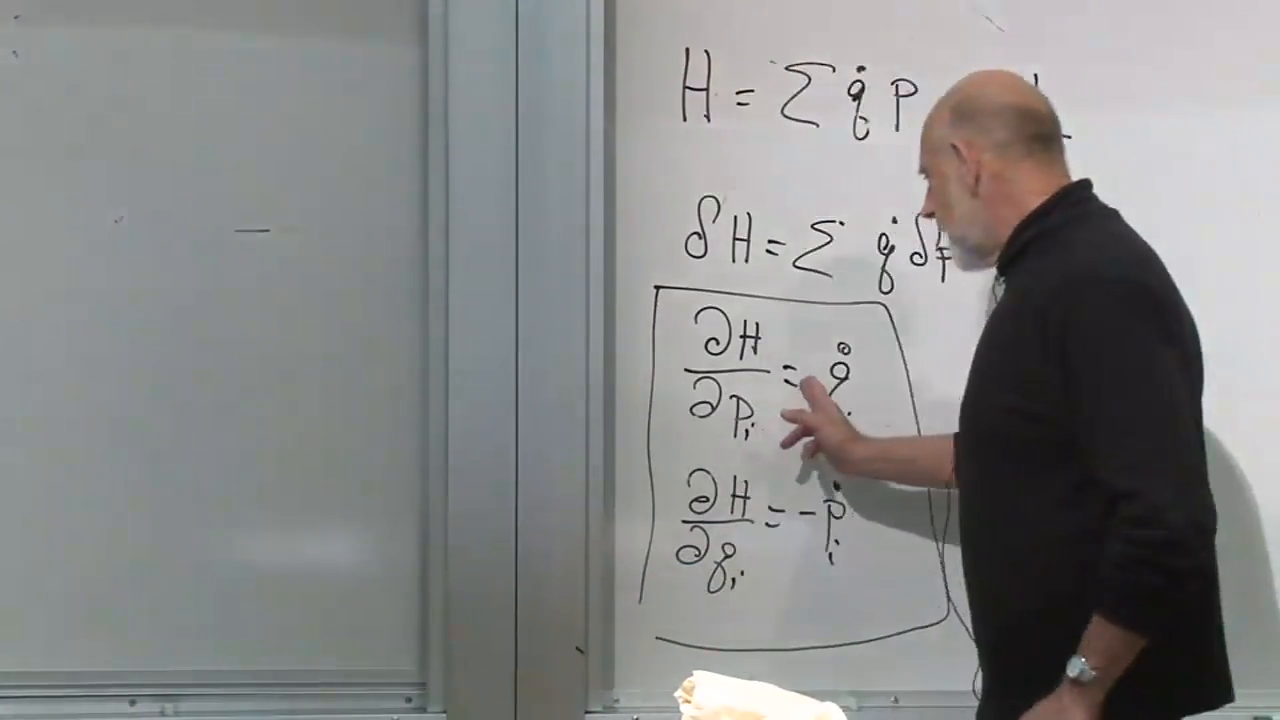
\includegraphics[width=0.78\textwidth]{lecture_06_figure_03.png}
  \caption{La definición del hamiltoniano, su variación y las ecuaciones canónicas enmarcadas.}
  \lectureframe{01:22:18}
\end{figure}

Para \(n\) coordenadas, estas son \(2n\) ecuaciones de primer orden. La formulación de Euler--Lagrange, en cambio, proporciona \(n\) ecuaciones de segundo orden. La cantidad de datos iniciales y el contenido físico son idénticos.

\section{El movimiento del oscilador como rotación rígida}

Al aplicar la ecuación~\eqref{eq:l6-hamilton-equations} a la ecuación~\eqref{eq:l6-oscillator-hamiltonian} se obtiene
\begin{equation}
  \dot q=\omega p,
  \qquad
  \dot p=-\omega q.
  \label{eq:l6-oscillator-first-order}
\end{equation}
Al derivar la primera ecuación y usar la segunda,
\begin{equation}
  \ddot q=\omega\dot p=-\omega^2q.
  \label{eq:l6-oscillator-second-order}
\end{equation}
Así, las dos ecuaciones de primer orden son exactamente la ecuación habitual del oscilador de segundo orden, junto con la definición del momento.

En el espacio de fases, el vector velocidad en \((q,p)\) es
\((\dot q,\dot p)=(\omega p,-\omega q)\), tangente al círculo de energía.
Cada radio gira con la misma velocidad angular \(\omega\). Podemos imaginar todo el plano como un molinillo rígido o como un fluido ficticio incompresible. Sus puntos circulan; no se comprimen hacia un sumidero ni se dispersan desde una fuente.

\begin{figure}[htbp]
  \centering
  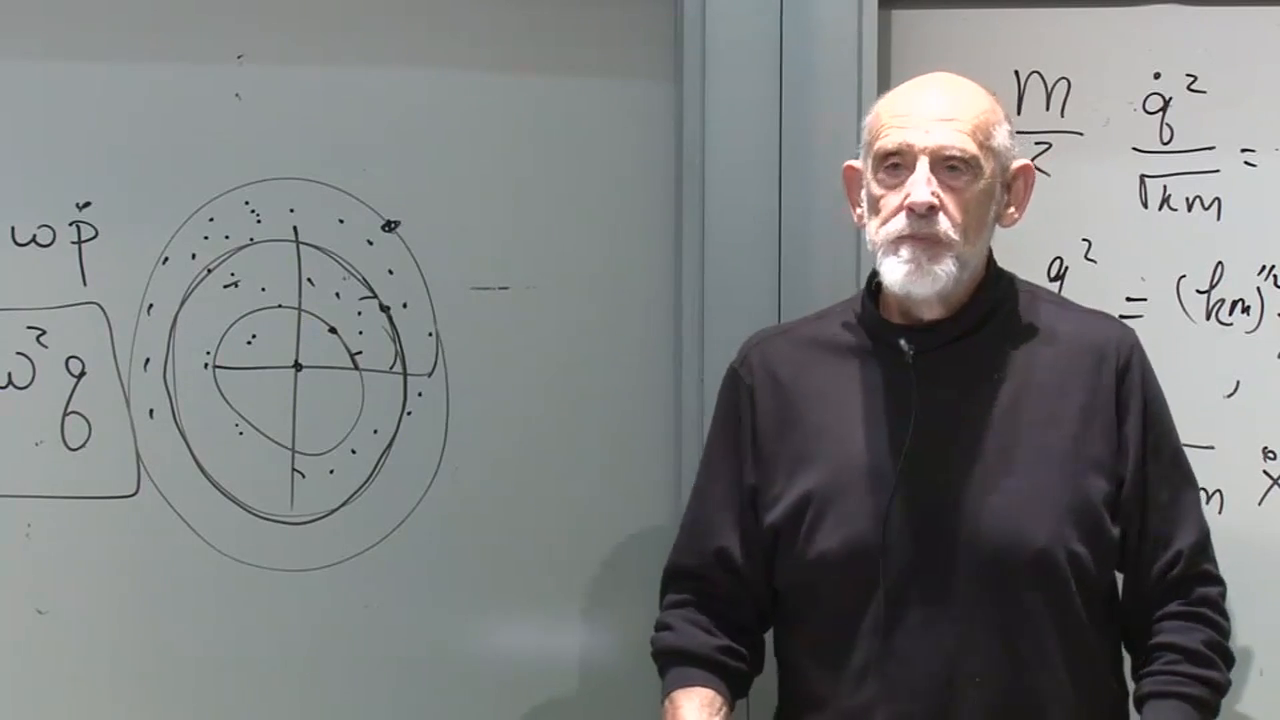
\includegraphics[width=0.86\textwidth]{lecture_06_figure_04.png}
  \caption{Una nube de puntos iniciales distribuida sobre trayectorias anidadas del espacio de fases. La evolución hamiltoniana desplaza la nube, en vez de hacerla colapsar en un estado preferido.}
  \lectureframe{01:39:27}
\end{figure}

\begin{figure}[htbp]
  \centering
  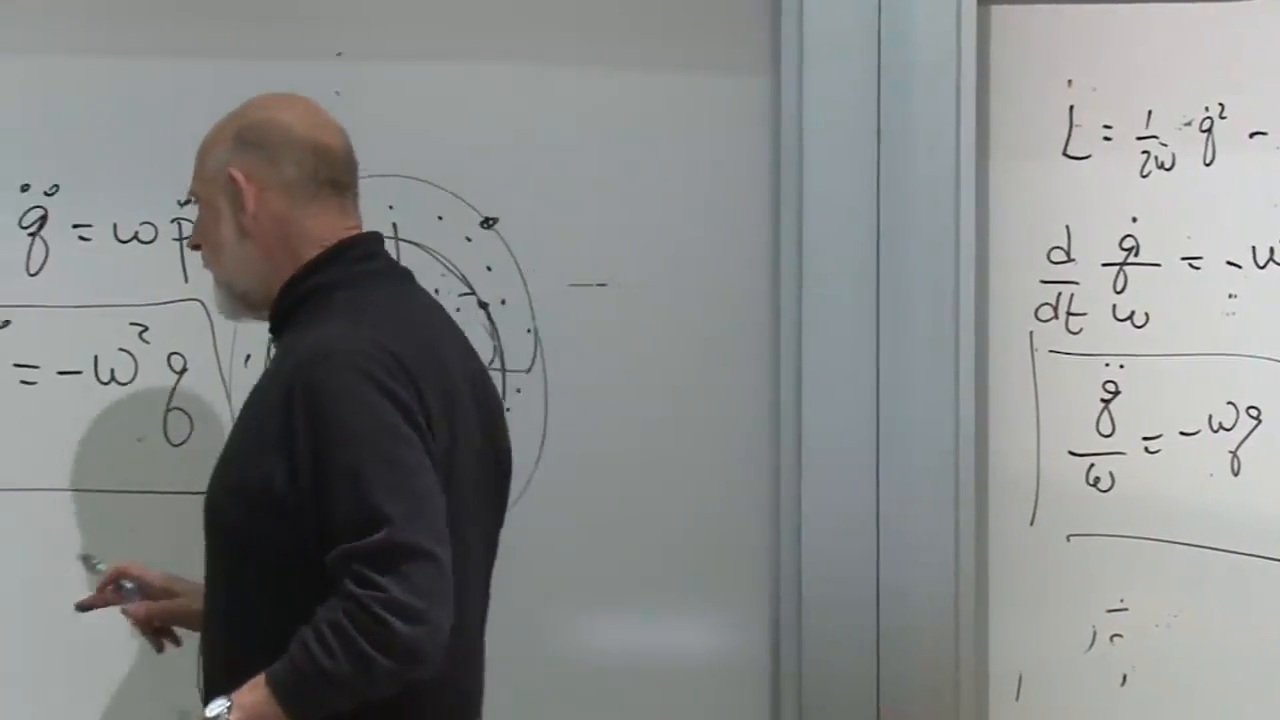
\includegraphics[width=0.90\textwidth]{lecture_06_figure_05.png}
  \caption{El retrato de fases del oscilador junto a la ecuación equivalente de Euler--Lagrange
  \(\ddot q/\omega=-\omega q\).}
  \lectureframe{01:42:10}
\end{figure}

El siguiente paso será convertir la analogía del fluido en un teorema: el flujo hamiltoniano no presenta convergencia ni divergencia local. Este resultado vuelve a conectar la mecánica continua con los mapas reversibles de estados que se estudiaron al comienzo del curso.

\section{Preguntas que ponen de manifiesto la elección de coordenadas}

\begin{classroomqa}
  \audiencequestion{¿Es un teorema o una propiedad empírica de los sistemas físicos la hipótesis de que se pueden despejar las velocidades en función de \(q\) y \(p\)?
  \lecturetimestamp{01:29:08--01:29:45}}
  \lecturerresponse{En este desarrollo elemental es una regularidad empírica, con una motivación más profunda en la mecánica cuántica. Más precisamente, la ecuación~\eqref{eq:l6-legendre-map} debe tener un jacobiano no singular respecto de las velocidades. La mecánica moderna también incluye lagrangianos singulares importantes, sobre todo en sistemas con restricciones y sistemas gauge, pero su formulación hamiltoniana requiere herramientas adicionales para tratar las restricciones.}
\end{classroomqa}

Una objeción sobre las unidades explica por qué el oscilador se escribió en la forma poco familiar de la ecuación~\eqref{eq:l6-rescaled-lagrangian}. Partamos, en cambio, de la coordenada habitual \(x\):
\begin{equation}
  L=\frac{m}{2}\dot x^2-\frac{k}{2}x^2,
  \qquad
  \omega=\sqrt{\frac{k}{m}}.
  \label{eq:l6-ordinary-oscillator}
\end{equation}
Elijamos
\begin{equation}
  q=(km)^{1/4}x.
  \label{eq:l6-oscillator-rescaling}
\end{equation}
Entonces, \(q^2=\sqrt{km}\,x^2\) y
\(\dot q^2=\sqrt{km}\,\dot x^2\), lo que transforma la ecuación~\eqref{eq:l6-ordinary-oscillator} precisamente en la ecuación~\eqref{eq:l6-rescaled-lagrangian}. La nueva \(q\) es una coordenada generalizada adaptada, no una longitud, y su conjugada \(p\) no es el momento mecánico ordinario \(p_x=m\dot x\).

\begin{figure}[htbp]
  \centering
  \includegraphics[width=0.86\textwidth]{lecture_06_figure_15.png}
  \caption{Reescalamiento dimensional desde la coordenada usual del oscilador \(x\) hasta la coordenada adaptada \(q=(km)^{1/4}x\).}
  \lectureframe{01:36:10}
\end{figure}

\begin{classroomqa}
  \audiencequestion{¿Cómo puede \(\omega p=\dot q\) ser dimensionalmente coherente y por qué se eligieron estas variables?
  \lecturetimestamp{01:29:46--01:39:22}}
  \lecturerresponse{El símbolo \(q\) no tiene por qué tener dimensiones de longitud, ni su conjugado \(p\) tiene por qué tener las dimensiones de \(m\dot x\). El reescalamiento de la ecuación~\eqref{eq:l6-oscillator-rescaling} conserva las dimensiones del lagrangiano y hace que \(q\) y \(p\) aparezcan simétricamente en \(H\). En las variables originales,
  \[
    H=\frac{p_x^2}{2m}+\frac{kx^2}{2},
  \]
  las curvas de energía constante en el plano \((x,p_x)\) son elipses. En el plano adaptado \((q,p)\) son círculos. El reescalamiento se eligió para hacer visible esa simetría.}
\end{classroomqa}

\begin{classroomqa}
  \audiencequestion{¿Cómo pueden ser equivalentes \(2n\) ecuaciones hamiltonianas de primer orden y \(n\) ecuaciones lagrangianas de segundo orden?
  \lecturetimestamp{01:39:24--01:42:30}}
  \lecturerresponse{Para el oscilador, derivemos \(\dot q=\omega p\) y sustituyamos \(\dot p=-\omega q\); el par se convierte en \(\ddot q=-\omega^2q\). Si partimos directamente del lagrangiano, obtenemos
  \[
    \frac{d}{dt}\left(\frac{\dot q}{\omega}\right)
      =-\omega q,
  \]
  que es la misma ecuación de segundo orden. Una de las ecuaciones de Hamilton puede interpretarse como la definición del momento en función de la velocidad, mientras que la otra determina la evolución de ese momento.}
\end{classroomqa}

\section{Por qué importan el espacio de fases y la energía potencial}

\begin{classroomqa}
  \audiencequestion{¿El poder del formalismo hamiltoniano significa que el espacio de fases es una representación geométrica mejor que el espacio de configuraciones?
  \lecturetimestamp{01:42:33--01:44:38}}
  \lecturerresponse{Sirven para propósitos distintos. El espacio de fases hace especialmente transparentes los ciclos, las superficies de energía constante y la ausencia de convergencia o divergencia. El espacio de configuraciones puede ser más adecuado para otras preguntas. La razón más profunda para destacar \(H\) es que se convierte en un objeto central y más intuitivo en la mecánica cuántica, una de las disciplinas modernas hacia las que se orienta este curso de mecánica.}
\end{classroomqa}

\begin{classroomqa}
  \audiencequestion{¿Debe considerarse la energía potencial como la integral de la fuerza?
  \lecturetimestamp{01:44:40--01:45:45}}
  \lecturerresponse{Para fuerzas conservativas, esa afirmación es válida, salvo una constante y con el signo correspondiente. Resulta más útil considerar el potencial como una magnitud primaria y derivar de él la fuerza generalizada:
  \[
    F_i=-\frac{\partial V}{\partial q_i}.
  \]
  Este es exactamente el término que aparece en \(\dot p_i=\partial L/\partial q_i\) cuando \(L=T-V\) y la energía cinética no depende explícitamente de \(q_i\).}
\end{classroomqa}

\begin{classroomqa}
  \audiencequestion{¿Hacia qué problemas de frontera de la física moderna conduce este camino?
  \lecturetimestamp{01:45:46--01:47:47}}
  \lecturerresponse{Este camino conduce a la gravedad cuántica y la cosmología; la física de partículas elementales, incluidos el sector de Higgs y los neutrinos; la relatividad; la teoría de cuerdas; y la teoría cuántica de campos. El problema teórico persistente consiste en integrar estas piezas en una estructura coherente, en particular la mecánica cuántica con la gravedad y la cosmología con la física de partículas. Esta era una descripción de la frontera tal como se presentaba en 2011, no una afirmación de que su solución ya se conociera.}
\end{classroomqa}

Los dos ejemplos con restricciones y el oscilador encajan ahora en un mismo esquema. Las coordenadas generalizadas eliminan fuerzas innecesarias. La simetría selecciona momentos canónicos conservados. La transformación de Legendre intercambia velocidades por momentos, y las ecuaciones de Hamilton convierten la dinámica en un flujo sobre el espacio de fases. En el caso del oscilador, ese flujo es una rotación rígida; para un sistema general, su geometría proporcionará el significado continuo preciso del movimiento reversible.